\RequirePackage{luatex85}
\documentclass[tikz]{standalone}
% Default preamble
\usepackage{pgfplots}
\pgfplotsset{compat=newest}
\usepgfplotslibrary{groupplots}
\usepgfplotslibrary{polar}
\usepgfplotslibrary{statistics}
\usepgfplotslibrary{dateplot}
% Custom preamble from global variable:
\usepackage{amsfonts}
\newcommand{\littletriangle}[1]
{
    \pgfplotsextra
    {
        \pgfkeysgetvalue{/pgfplots/xmin}{\xmin}
        \pgfkeysgetvalue{/pgfplots/xmax}{\xmax}
        \pgfkeysgetvalue{/pgfplots/ymin}{\ymin}
        \pgfkeysgetvalue{/pgfplots/ymax}{\ymax}

        \pgfmathsetmacro{\xArel}{0.25}
        \pgfmathsetmacro{\yArel}{0.1}
        \pgfmathsetmacro{\xBrel}{0.1}
        \pgfmathsetmacro{\yBrel}{\yArel}
        \pgfmathsetmacro{\xCrel}{\xBrel}

        \pgfmathsetmacro{\lnxB}{\xmin*(1-(0.1))+\xmax*(0.1)}
        \pgfmathsetmacro{\lnxA}{\xmin*(1-0.25)+\xmax*0.25}
        \pgfmathsetmacro{\lnyA}{\ymin*(1-0.1)+\ymax*0.1}
        \pgfmathsetmacro{\lnyC}{\lnyA+#1*(\lnxA-\lnxB)}
        \pgfmathsetmacro{\yCrel}{\lnyC-\ymin)/(\ymax-\ymin)}
        
        \coordinate (A) at (rel axis cs:\xArel,\yArel);
        \coordinate (B) at (rel axis cs:\xBrel,\yBrel);
        \coordinate (C) at (rel axis cs:\xCrel,\yCrel);

        \draw[black]   (A)--node[pos=0.9,yshift=1ex,xshift=0.5ex] {\small #1}
                    (B)--
                    (C)-- 
                    cycle;
    }
}

\newcommand{\drawsquare}[3]{\draw[thick,black,fill=#3] (#1,#2)--(#1,#2+1)--(#1+1,#2+1)--(#1+1,#2)--cycle;}


\begin{document}
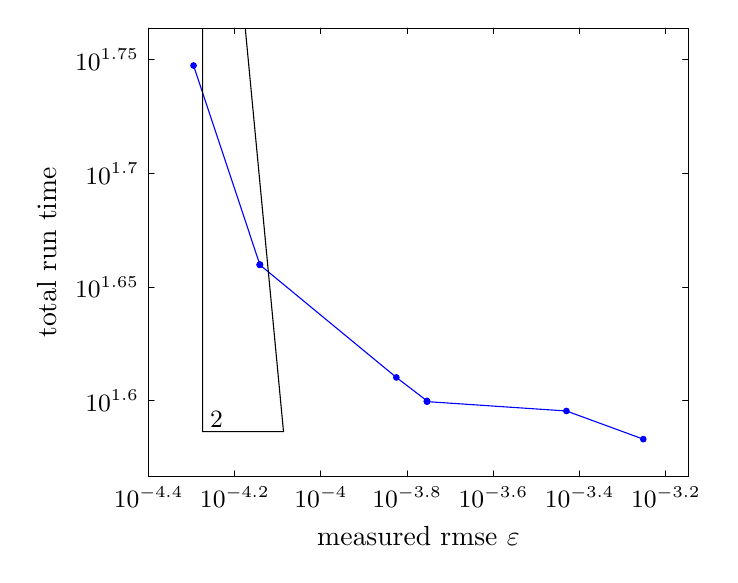
\begin{tikzpicture}
\begin{axis}[ticklabel style={{font=\small}}, major tick length={2pt}, every tick/.style={{black, line cap=round}}, axis on top, legend style={{draw=none, font=\small, at={(0.03,0.03)}, anchor=south west, fill=none, legend cell align=left}}, xmode={log}, ymode={log}, legend style={{draw=none, font=\small, at={(0.97,0.97)}, anchor=north east, fill=none, legend cell align=left}}, xlabel={measured rmse $\varepsilon$}, ylabel={total run time}]
    \addplot[mark={*}, mark size={1pt}, line cap={round}, mark options={solid}, color={blue}]
        table[row sep={\\}]
        {
            \\
            0.0005594264185554075  38.310346175  \\
            0.00037114552272392325  39.413315241  \\
            0.00017624486309656654  39.790634082  \\
            0.00017624486309656654  39.798099349999994  \\
            0.00017624486309656654  39.82085766099999  \\
            0.00014962231128500412  40.77298035399999  \\
            7.217014558150605e-5  45.695573018999994  \\
            7.217014558150605e-5  45.702916867999996  \\
            7.217014558150605e-5  45.71073394  \\
            5.0650836988525666e-5  55.919780277  \\
        }
        ;
    \littletriangle{2};
\end{axis}
\end{tikzpicture}
\end{document}
